\begin{center}
    \textbf{\titlePageTypeWork~№\titlePageNumberWork}
\end{center}

\textbf{Тема}: "\titlePageTopic".

\textbf{Цель}: 

\begin{center}
    \textbf{Ход работы}:
\end{center}

\subparagraph{Задание для выполнения}
Написать программу, которая будет реализовывать следующие функции:
\begin{itemize}
\item сразу после запуска получает и сообщает свой ID и ID родительского процесса;
\item перед каждым выводом сообщения об ID процесса и родительского процесса эта информация получается заново;
\item порождает процессы, формируя генеалогическое дерево согласно варианту, сообщая, что "процесс с ID таким-то породил процесс с таким-то ID";
\item перед завершением процесса сообщить, что "процесс с таким-то ID и таким-то ID родителя завершает работу";
\item один из процессов должен вместо себя запустить программу, указанную в варианте задания.
\end{itemize}

На основании выходной информации программы предыдущего пункта изобразить генеалогическое дерево процессов (с указанием идентификаторов процессов).
Объяснить каждое выведенное сообщение и их порядок в предыдущем пункте.

\subparagraph{Варианты индивидуальных заданий}
В столбце fork описано генеалогическое древо процессов: каждая цифра указывает на относительный номер (не путать с pid) процесса, являющегося родителем для данного процесса. 
Например, строка 0 1 1 1 3 означает, что первый процесс не имеет родителя среди ваших процессов (порождается и запускается извне), второй, третий и четвертый - порождены первым, пятый - третьим.
В столбце exec указан номер процесса, выполняющего вызов exec, команды для которого указаны в последнем столбце.
Запускайте команду обязательно с какими-либо параметрами.

\begin{table}[!htp]
    \centering
    \caption{Вариант 5}
    \begin{tabular}{|l|l|l|}
        \hline
        No  & fork              & exec  \\  \hline
        \hline
        5   & 0 1 1 2 2 3 3 5   & df    \\  \hline
    \end{tabular}
\end{table}

\newpage

\textbf{Вариант 5}

\lstinputlisting[
    name=main.c,
    language=C++,
    basicstyle=\ttfamily\scriptsize,
]
{../../src/option5/app/main.c}

\begin{figure}[!htp]
    \begin{minipage}{0.49\textwidth}
        \centering
        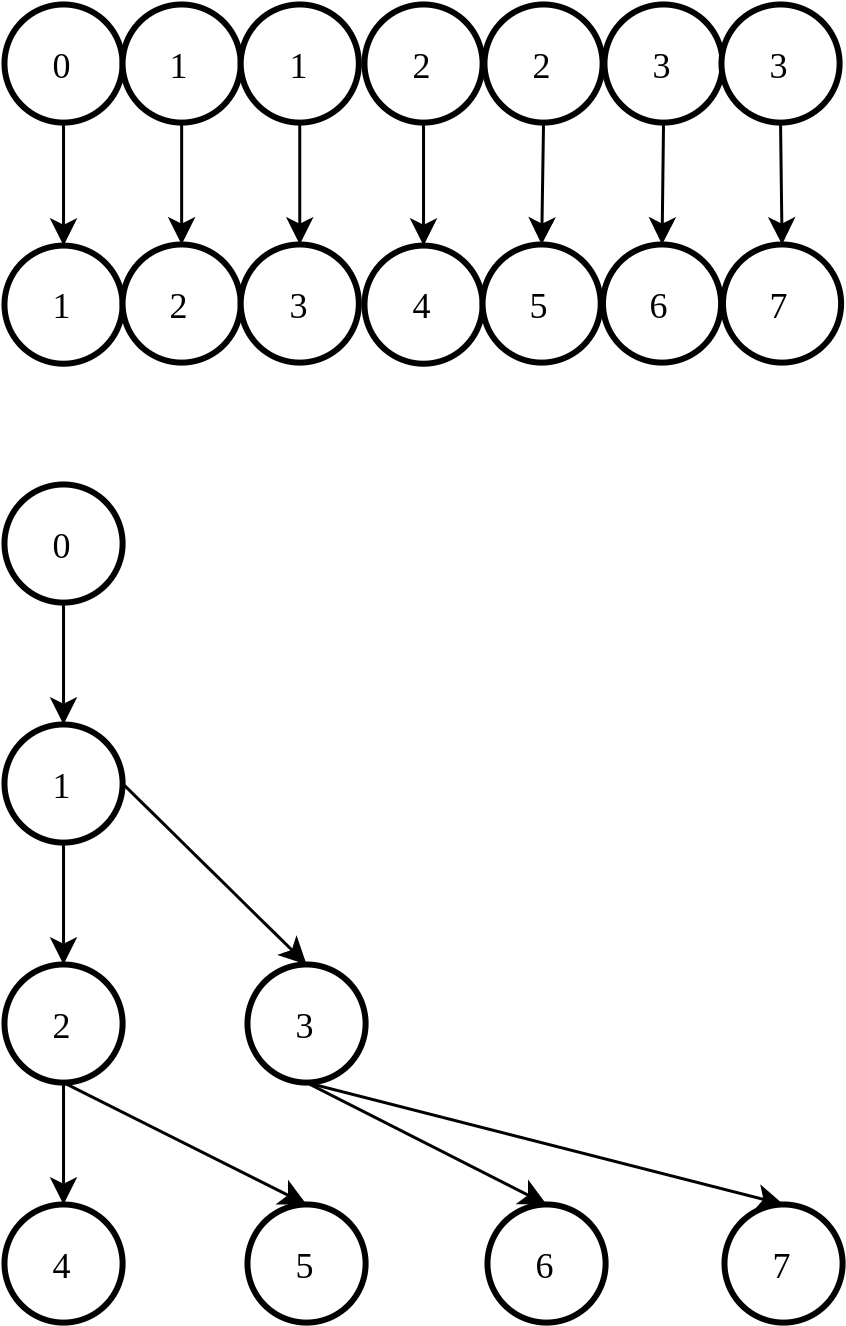
\includegraphics[height=6.6cm]
        {../_INCLUDES/option5/option5.png}
        \caption{Генелогическое дерево варианта 5}
    \end{minipage}\hfill
    \begin{minipage}{0.49\textwidth}
        \centering
        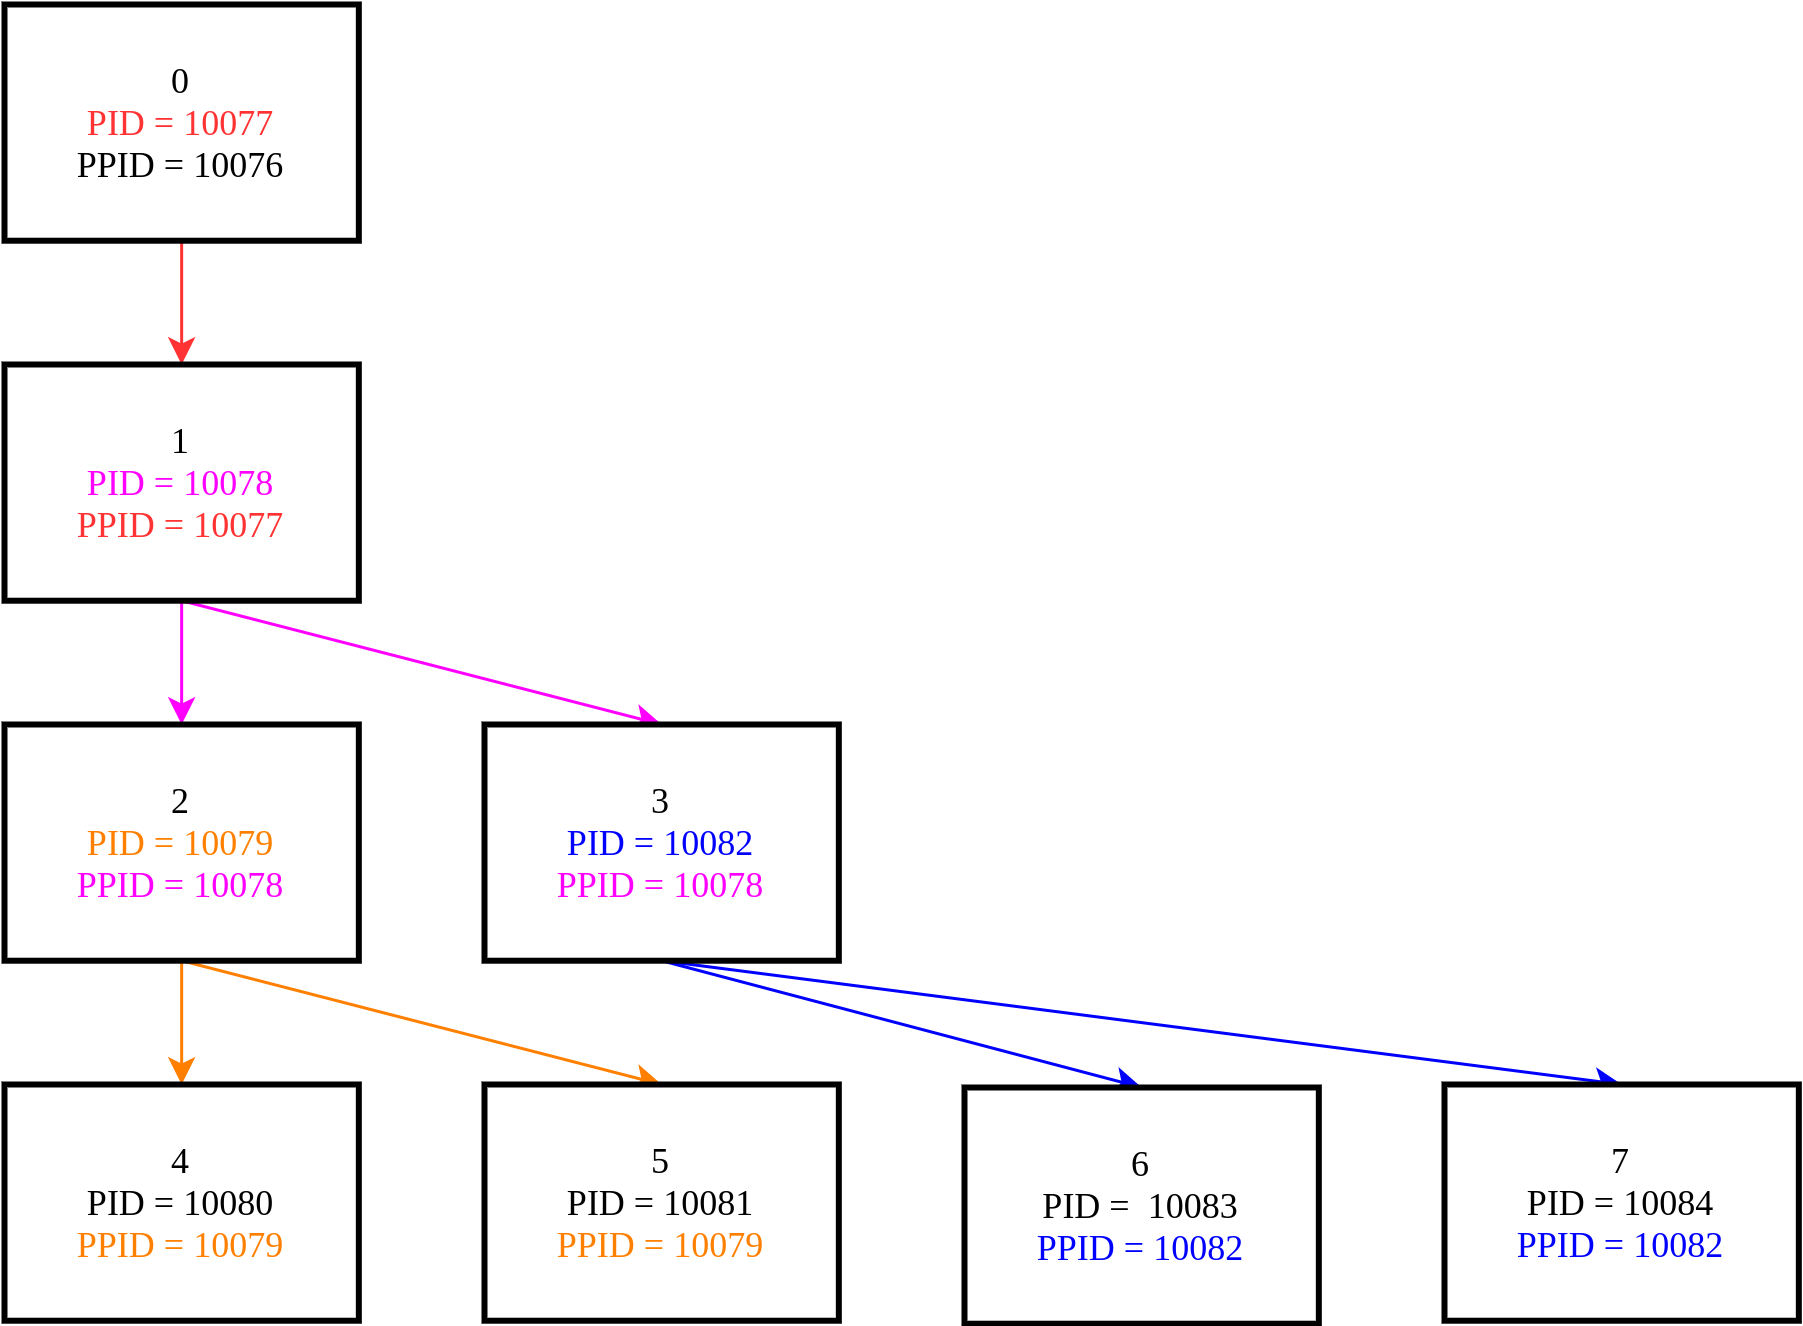
\includegraphics[height=6.6cm]
        {../_INCLUDES/option5/option5-test.png}
        \caption{Проверка генелогического дерева}
    \end{minipage}
\end{figure}

\newpage

\begin{lstlisting}[
    language=Out,
    basicstyle=\ttfamily\scriptsize,
]
start pr 0 PID = 8661 PPID = 8660
	start pr 1 PID = 8662 PPID = 8661
		start pr 2 PID = 8663 PPID = 8662
			start pr 4 PID = 8664 PPID = 8663
			end pr 4
			start pr 5 PID = 8665 PPID = 8663
		end and exec(df) pr 5

				= = = = = run $df
Filesystem     1K-blocks     Used Available Use% Mounted on
udev             1905716        0   1905716   0% /dev
tmpfs             387056     1636    385420   1% /run
/dev/sda5       28705700 17692176   9532308  65% /
tmpfs            1935264    20108   1915156   2% /dev/shm
tmpfs               5120        4      5116   1% /run/lock
tmpfs            1935264        0   1935264   0% /sys/fs/cgroup
/dev/loop0         56832    56832         0 100% /snap/core18/1988
/dev/loop1        134784   134784         0 100% /snap/docker/796
/dev/loop2         33152    33152         0 100% /snap/snapd/11107
/dev/loop3         33152    33152         0 100% /snap/snapd/11402
/dev/sda1          98304    36511     61793  38% /boot/efi
/dev/sda6      165168784 65692132  91016828  42% /home
tmpfs             387052       44    387008   1% /run/user/1000
		start pr 3 PID = 8666 PPID = 8662
			start pr 6 PID = 8667 PPID = 8666
			end pr 6
			start pr 7 PID = 8668 PPID = 8666
			end pr 7
		end pr 3
	end pr 1
End program...
\end{lstlisting}
